\hypertarget{group__xEventGroupWaitBits}{}\section{x\+Event\+Group\+Wait\+Bits}
\label{group__xEventGroupWaitBits}\index{x\+Event\+Group\+Wait\+Bits@{x\+Event\+Group\+Wait\+Bits}}
Collaboration diagram for x\+Event\+Group\+Wait\+Bits\+:\nopagebreak
\begin{figure}[H]
\begin{center}
\leavevmode
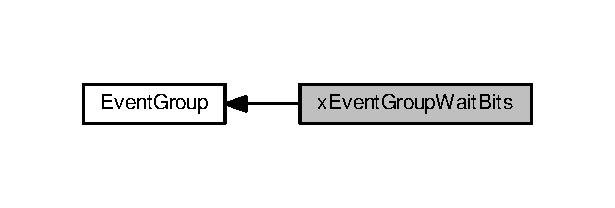
\includegraphics[width=295pt]{d6/d9a/group__xEventGroupWaitBits}
\end{center}
\end{figure}
\hyperlink{event__groups_8h}{event\+\_\+groups.\+h} 
\begin{DoxyPre}
EventGroupHandle\_t xEventGroupCreateStatic( EventGroupHandle\_t * pxEventGroupBuffer );
\end{DoxyPre}


Create a new event group.

Internally, within the Free\+R\+T\+OS implementation, event groups use a \mbox{[}small\mbox{]} block of memory, in which the event group\textquotesingle{}s structure is stored. If an event groups is created using x\+Event\+Gropu\+Create() then the required memory is automatically dynamically allocated inside the x\+Event\+Group\+Create() function. (see \href{http://www.freertos.org/a00111.html}{\tt http\+://www.\+freertos.\+org/a00111.\+html}). If an event group is created using x\+Event\+Gropu\+Create\+Static() then the application writer must instead provide the memory that will get used by the event group. x\+Event\+Group\+Create\+Static() therefore allows an event group to be created without using any dynamic memory allocation.

Although event groups are not related to ticks, for internal implementation reasons the number of bits available for use in an event group is dependent on the config\+U\+S\+E\+\_\+16\+\_\+\+B\+I\+T\+\_\+\+T\+I\+C\+KS setting in \hyperlink{FreeRTOSConfig_8h}{Free\+R\+T\+O\+S\+Config.\+h}. If config\+U\+S\+E\+\_\+16\+\_\+\+B\+I\+T\+\_\+\+T\+I\+C\+KS is 1 then each event group contains 8 usable bits (bit 0 to bit 7). If config\+U\+S\+E\+\_\+16\+\_\+\+B\+I\+T\+\_\+\+T\+I\+C\+KS is set to 0 then each event group has 24 usable bits (bit 0 to bit 23). The Event\+Bits\+\_\+t type is used to store event bits within an event group.


\begin{DoxyParams}{Parameters}
{\em px\+Event\+Group\+Buffer} & px\+Event\+Group\+Buffer must point to a variable of type Static\+Event\+Group\+\_\+t, which will be then be used to hold the event group\textquotesingle{}s data structures, removing the need for the memory to be allocated dynamically.\\
\hline
\end{DoxyParams}
\begin{DoxyReturn}{Returns}
If the event group was created then a handle to the event group is returned. If px\+Event\+Group\+Buffer was N\+U\+LL then N\+U\+LL is returned.
\end{DoxyReturn}
Example usage\+: 
\begin{DoxyPre}
   // StaticEventGroup\_t is a publicly accessible structure that has the same
   // size and alignment requirements as the real event group structure.  It is
   // provided as a mechanism for applications to know the size of the event
   // group (which is dependent on the architecture and configuration file
   // settings) without breaking the strict data hiding policy by exposing the
   // real event group internals.  This StaticEventGroup\_t variable is passed
   // into the xSemaphoreCreateEventGroupStatic() function and is used to store
   // the event group's data structures
   StaticEventGroup\_t xEventGroupBuffer;\end{DoxyPre}



\begin{DoxyPre}   // Create the event group without dynamically allocating any memory.
   xEventGroup = xEventGroupCreateStatic( &xEventGroupBuffer );
  \end{DoxyPre}
 \hyperlink{event__groups_8h}{event\+\_\+groups.\+h} 
\begin{DoxyPre}
   EventBits\_t xEventGroupWaitBits(     EventGroupHandle\_t xEventGroup,
                                    const EventBits\_t uxBitsToWaitFor,
                                    const BaseType\_t xClearOnExit,
                                    const BaseType\_t xWaitForAllBits,
                                    const TickType\_t xTicksToWait );
\end{DoxyPre}


\mbox{[}Potentially\mbox{]} block to wait for one or more bits to be set within a previously created event group.

This function cannot be called from an interrupt.


\begin{DoxyParams}{Parameters}
{\em x\+Event\+Group} & The event group in which the bits are being tested. The event group must have previously been created using a call to x\+Event\+Group\+Create().\\
\hline
{\em ux\+Bits\+To\+Wait\+For} & A bitwise value that indicates the bit or bits to test inside the event group. For example, to wait for bit 0 and/or bit 2 set ux\+Bits\+To\+Wait\+For to 0x05. To wait for bits 0 and/or bit 1 and/or bit 2 set ux\+Bits\+To\+Wait\+For to 0x07. Etc.\\
\hline
{\em x\+Clear\+On\+Exit} & If x\+Clear\+On\+Exit is set to pd\+T\+R\+UE then any bits within ux\+Bits\+To\+Wait\+For that are set within the event group will be cleared before \hyperlink{event__groups_8h_aab9d5b405bc57b7624dcabe9a9a503db}{x\+Event\+Group\+Wait\+Bits()} returns if the wait condition was met (if the function returns for a reason other than a timeout). If x\+Clear\+On\+Exit is set to pd\+F\+A\+L\+SE then the bits set in the event group are not altered when the call to \hyperlink{event__groups_8h_aab9d5b405bc57b7624dcabe9a9a503db}{x\+Event\+Group\+Wait\+Bits()} returns.\\
\hline
{\em x\+Wait\+For\+All\+Bits} & If x\+Wait\+For\+All\+Bits is set to pd\+T\+R\+UE then \hyperlink{event__groups_8h_aab9d5b405bc57b7624dcabe9a9a503db}{x\+Event\+Group\+Wait\+Bits()} will return when either all the bits in ux\+Bits\+To\+Wait\+For are set or the specified block time expires. If x\+Wait\+For\+All\+Bits is set to pd\+F\+A\+L\+SE then \hyperlink{event__groups_8h_aab9d5b405bc57b7624dcabe9a9a503db}{x\+Event\+Group\+Wait\+Bits()} will return when any one of the bits set in ux\+Bits\+To\+Wait\+For is set or the specified block time expires. The block time is specified by the x\+Ticks\+To\+Wait parameter.\\
\hline
{\em x\+Ticks\+To\+Wait} & The maximum amount of time (specified in \textquotesingle{}ticks\textquotesingle{}) to wait for one/all (depending on the x\+Wait\+For\+All\+Bits value) of the bits specified by ux\+Bits\+To\+Wait\+For to become set.\\
\hline
\end{DoxyParams}
\begin{DoxyReturn}{Returns}
The value of the event group at the time either the bits being waited for became set, or the block time expired. Test the return value to know which bits were set. If \hyperlink{event__groups_8h_aab9d5b405bc57b7624dcabe9a9a503db}{x\+Event\+Group\+Wait\+Bits()} returned because its timeout expired then not all the bits being waited for will be set. If \hyperlink{event__groups_8h_aab9d5b405bc57b7624dcabe9a9a503db}{x\+Event\+Group\+Wait\+Bits()} returned because the bits it was waiting for were set then the returned value is the event group value before any bits were automatically cleared in the case that x\+Clear\+On\+Exit parameter was set to pd\+T\+R\+UE.
\end{DoxyReturn}
Example usage\+: 
\begin{DoxyPre}
  #define BIT\_0 ( 1 << 0 )
  #define BIT\_4 ( 1 << 4 )\end{DoxyPre}



\begin{DoxyPre}  void aFunction( EventGroupHandle\_t xEventGroup )
  \{
  EventBits\_t uxBits;
  const TickType\_t xTicksToWait = 100 / portTICK\_PERIOD\_MS;\end{DoxyPre}



\begin{DoxyPre}    // Wait a maximum of 100ms for either bit 0 or bit 4 to be set within
    // the event group.  Clear the bits before exiting.
    uxBits = xEventGroupWaitBits(
                xEventGroup,    // The event group being tested.
                BIT\_0 | BIT\_4,  // The bits within the event group to wait for.
                pdTRUE,         // BIT\_0 and BIT\_4 should be cleared before returning.
                pdFALSE,        // Don't wait for both bits, either bit will do.
                xTicksToWait ); // Wait a maximum of 100ms for either bit to be set.\end{DoxyPre}



\begin{DoxyPre}    if( ( uxBits \& ( BIT\_0 | BIT\_4 ) ) == ( BIT\_0 | BIT\_4 ) )
    \{
        // \hyperlink{event__groups_8h_aab9d5b405bc57b7624dcabe9a9a503db}{xEventGroupWaitBits()} returned because both bits were set.
    \}
    else if( ( uxBits \& BIT\_0 ) != 0 )
    \{
        // \hyperlink{event__groups_8h_aab9d5b405bc57b7624dcabe9a9a503db}{xEventGroupWaitBits()} returned because just BIT\_0 was set.
    \}
    else if( ( uxBits \& BIT\_4 ) != 0 )
    \{
        // \hyperlink{event__groups_8h_aab9d5b405bc57b7624dcabe9a9a503db}{xEventGroupWaitBits()} returned because just BIT\_4 was set.
    \}
    else
    \{
        // \hyperlink{event__groups_8h_aab9d5b405bc57b7624dcabe9a9a503db}{xEventGroupWaitBits()} returned because xTicksToWait ticks passed
        // without either BIT\_0 or BIT\_4 becoming set.
    \}
  \}
  \end{DoxyPre}
 